% Per-kernel augmentation status heatmap — CUDA-to-OMP, Qwen 3.5 397B
% Exact data provided by user (matches pre-phase-3 augmentation_analysis output).
% Groups: stable_pass (rows 0-17) | degradation (18-21) | stable_fail (22-23).
% Colors: Okabe-Ito palette matching augmentation_analysis.py.

\definecolor{augPass}{RGB}{0,158,115}      % teal-green  (PASS)
\definecolor{augBF}{RGB}{213,94,0}         % vermillion  (BUILD_FAIL)
\definecolor{augEF}{RGB}{204,121,167}      % pink/lavender (EXTRACTION_FAIL)
\definecolor{augMissing}{RGB}{220,220,220} % light gray   (not used here)

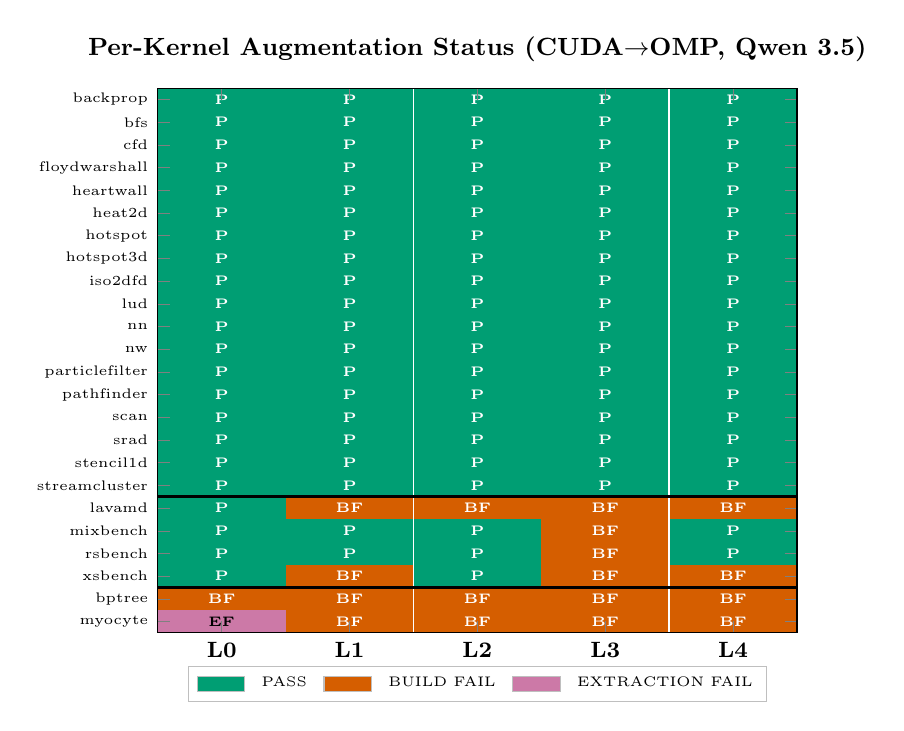
\begin{tikzpicture}
\begin{axis}[
  width=0.80\columnwidth,
  height=8.5cm,
  enlargelimits=false,
  axis on top,
  xmin=-0.5, xmax=4.5,
  ymin=-0.5, ymax=23.5,
  y dir=reverse,
  xtick={0,1,2,3,4},
  xticklabels={L0, L1, L2, L3, L4},
  x tick label style={font=\footnotesize\bfseries},
  ytick={0,1,2,3,4,5,6,7,8,9,10,11,12,13,14,15,16,17,18,19,20,21,22,23},
  yticklabels={
    backprop, bfs, cfd, floydwarshall, heartwall, heat2d,
    hotspot, hotspot3d, iso2dfd, lud, nn, nw,
    particlefilter, pathfinder, scan, srad, stencil1d, streamcluster,
    lavamd, mixbench, rsbench, xsbench,
    bptree, myocyte
  },
  y tick label style={font=\tiny, anchor=east},
  title style={font=\small\bfseries, align=center},
  title={Per-Kernel Augmentation Status (CUDA$\to$OMP, Qwen~3.5)},
  legend style={
    at={(0.5,-0.06)}, anchor=north,
    font=\tiny, draw=gray!50,
    legend columns=3, column sep=4pt,
  },
  clip=false,
]

% ---- Cell fills ----
% Rows 0-17: all PASS (stable_pass group)
\fill[augPass] (axis cs:-0.5,-0.5) rectangle (axis cs:4.5,17.5);

% Row 18 — lavamd: P BF BF BF BF
\fill[augPass] (axis cs:-0.5,17.5) rectangle (axis cs:0.5,18.5);
\fill[augBF]   (axis cs:0.5,17.5)  rectangle (axis cs:4.5,18.5);

% Row 19 — mixbench: P P P BF P
\fill[augPass] (axis cs:-0.5,18.5) rectangle (axis cs:0.5,19.5);
\fill[augPass] (axis cs:0.5,18.5)  rectangle (axis cs:1.5,19.5);
\fill[augPass] (axis cs:1.5,18.5)  rectangle (axis cs:2.5,19.5);
\fill[augBF]   (axis cs:2.5,18.5)  rectangle (axis cs:3.5,19.5);
\fill[augPass] (axis cs:3.5,18.5)  rectangle (axis cs:4.5,19.5);

% Row 20 — rsbench: P P P BF P
\fill[augPass] (axis cs:-0.5,19.5) rectangle (axis cs:0.5,20.5);
\fill[augPass] (axis cs:0.5,19.5)  rectangle (axis cs:1.5,20.5);
\fill[augPass] (axis cs:1.5,19.5)  rectangle (axis cs:2.5,20.5);
\fill[augBF]   (axis cs:2.5,19.5)  rectangle (axis cs:3.5,20.5);
\fill[augPass] (axis cs:3.5,19.5)  rectangle (axis cs:4.5,20.5);

% Row 21 — xsbench: P BF P BF BF
\fill[augPass] (axis cs:-0.5,20.5) rectangle (axis cs:0.5,21.5);
\fill[augBF]   (axis cs:0.5,20.5)  rectangle (axis cs:1.5,21.5);
\fill[augPass] (axis cs:1.5,20.5)  rectangle (axis cs:2.5,21.5);
\fill[augBF]   (axis cs:2.5,20.5)  rectangle (axis cs:3.5,21.5);
\fill[augBF]   (axis cs:3.5,20.5)  rectangle (axis cs:4.5,21.5);

% Row 22 — bptree: BF BF BF BF BF
\fill[augBF] (axis cs:-0.5,21.5) rectangle (axis cs:4.5,22.5);

% Row 23 — myocyte: EF BF BF BF BF
\fill[augEF]  (axis cs:-0.5,22.5) rectangle (axis cs:0.5,23.5);
\fill[augBF]  (axis cs:0.5,22.5)  rectangle (axis cs:4.5,23.5);

% ---- White grid lines ----
\draw[white, line width=0.5pt]
  (axis cs:-0.5,-0.5) grid[xstep=1, ystep=1] (axis cs:4.5,23.5);

% ---- Group separator lines ----
\draw[black, line width=1.2pt] (axis cs:-0.5,17.5) -- (axis cs:4.5,17.5);
\draw[black, line width=1.2pt] (axis cs:-0.5,21.5) -- (axis cs:4.5,21.5);

% ---- Cell labels ----
% Rows 0-17: all P (white text on green)
\node[font=\tiny\bfseries, text=white] at (axis cs:0,0)  {P}; \node[font=\tiny\bfseries, text=white] at (axis cs:1,0)  {P}; \node[font=\tiny\bfseries, text=white] at (axis cs:2,0)  {P}; \node[font=\tiny\bfseries, text=white] at (axis cs:3,0)  {P}; \node[font=\tiny\bfseries, text=white] at (axis cs:4,0)  {P};
\node[font=\tiny\bfseries, text=white] at (axis cs:0,1)  {P}; \node[font=\tiny\bfseries, text=white] at (axis cs:1,1)  {P}; \node[font=\tiny\bfseries, text=white] at (axis cs:2,1)  {P}; \node[font=\tiny\bfseries, text=white] at (axis cs:3,1)  {P}; \node[font=\tiny\bfseries, text=white] at (axis cs:4,1)  {P};
\node[font=\tiny\bfseries, text=white] at (axis cs:0,2)  {P}; \node[font=\tiny\bfseries, text=white] at (axis cs:1,2)  {P}; \node[font=\tiny\bfseries, text=white] at (axis cs:2,2)  {P}; \node[font=\tiny\bfseries, text=white] at (axis cs:3,2)  {P}; \node[font=\tiny\bfseries, text=white] at (axis cs:4,2)  {P};
\node[font=\tiny\bfseries, text=white] at (axis cs:0,3)  {P}; \node[font=\tiny\bfseries, text=white] at (axis cs:1,3)  {P}; \node[font=\tiny\bfseries, text=white] at (axis cs:2,3)  {P}; \node[font=\tiny\bfseries, text=white] at (axis cs:3,3)  {P}; \node[font=\tiny\bfseries, text=white] at (axis cs:4,3)  {P};
\node[font=\tiny\bfseries, text=white] at (axis cs:0,4)  {P}; \node[font=\tiny\bfseries, text=white] at (axis cs:1,4)  {P}; \node[font=\tiny\bfseries, text=white] at (axis cs:2,4)  {P}; \node[font=\tiny\bfseries, text=white] at (axis cs:3,4)  {P}; \node[font=\tiny\bfseries, text=white] at (axis cs:4,4)  {P};
\node[font=\tiny\bfseries, text=white] at (axis cs:0,5)  {P}; \node[font=\tiny\bfseries, text=white] at (axis cs:1,5)  {P}; \node[font=\tiny\bfseries, text=white] at (axis cs:2,5)  {P}; \node[font=\tiny\bfseries, text=white] at (axis cs:3,5)  {P}; \node[font=\tiny\bfseries, text=white] at (axis cs:4,5)  {P};
\node[font=\tiny\bfseries, text=white] at (axis cs:0,6)  {P}; \node[font=\tiny\bfseries, text=white] at (axis cs:1,6)  {P}; \node[font=\tiny\bfseries, text=white] at (axis cs:2,6)  {P}; \node[font=\tiny\bfseries, text=white] at (axis cs:3,6)  {P}; \node[font=\tiny\bfseries, text=white] at (axis cs:4,6)  {P};
\node[font=\tiny\bfseries, text=white] at (axis cs:0,7)  {P}; \node[font=\tiny\bfseries, text=white] at (axis cs:1,7)  {P}; \node[font=\tiny\bfseries, text=white] at (axis cs:2,7)  {P}; \node[font=\tiny\bfseries, text=white] at (axis cs:3,7)  {P}; \node[font=\tiny\bfseries, text=white] at (axis cs:4,7)  {P};
\node[font=\tiny\bfseries, text=white] at (axis cs:0,8)  {P}; \node[font=\tiny\bfseries, text=white] at (axis cs:1,8)  {P}; \node[font=\tiny\bfseries, text=white] at (axis cs:2,8)  {P}; \node[font=\tiny\bfseries, text=white] at (axis cs:3,8)  {P}; \node[font=\tiny\bfseries, text=white] at (axis cs:4,8)  {P};
\node[font=\tiny\bfseries, text=white] at (axis cs:0,9)  {P}; \node[font=\tiny\bfseries, text=white] at (axis cs:1,9)  {P}; \node[font=\tiny\bfseries, text=white] at (axis cs:2,9)  {P}; \node[font=\tiny\bfseries, text=white] at (axis cs:3,9)  {P}; \node[font=\tiny\bfseries, text=white] at (axis cs:4,9)  {P};
\node[font=\tiny\bfseries, text=white] at (axis cs:0,10) {P}; \node[font=\tiny\bfseries, text=white] at (axis cs:1,10) {P}; \node[font=\tiny\bfseries, text=white] at (axis cs:2,10) {P}; \node[font=\tiny\bfseries, text=white] at (axis cs:3,10) {P}; \node[font=\tiny\bfseries, text=white] at (axis cs:4,10) {P};
\node[font=\tiny\bfseries, text=white] at (axis cs:0,11) {P}; \node[font=\tiny\bfseries, text=white] at (axis cs:1,11) {P}; \node[font=\tiny\bfseries, text=white] at (axis cs:2,11) {P}; \node[font=\tiny\bfseries, text=white] at (axis cs:3,11) {P}; \node[font=\tiny\bfseries, text=white] at (axis cs:4,11) {P};
\node[font=\tiny\bfseries, text=white] at (axis cs:0,12) {P}; \node[font=\tiny\bfseries, text=white] at (axis cs:1,12) {P}; \node[font=\tiny\bfseries, text=white] at (axis cs:2,12) {P}; \node[font=\tiny\bfseries, text=white] at (axis cs:3,12) {P}; \node[font=\tiny\bfseries, text=white] at (axis cs:4,12) {P};
\node[font=\tiny\bfseries, text=white] at (axis cs:0,13) {P}; \node[font=\tiny\bfseries, text=white] at (axis cs:1,13) {P}; \node[font=\tiny\bfseries, text=white] at (axis cs:2,13) {P}; \node[font=\tiny\bfseries, text=white] at (axis cs:3,13) {P}; \node[font=\tiny\bfseries, text=white] at (axis cs:4,13) {P};
\node[font=\tiny\bfseries, text=white] at (axis cs:0,14) {P}; \node[font=\tiny\bfseries, text=white] at (axis cs:1,14) {P}; \node[font=\tiny\bfseries, text=white] at (axis cs:2,14) {P}; \node[font=\tiny\bfseries, text=white] at (axis cs:3,14) {P}; \node[font=\tiny\bfseries, text=white] at (axis cs:4,14) {P};
\node[font=\tiny\bfseries, text=white] at (axis cs:0,15) {P}; \node[font=\tiny\bfseries, text=white] at (axis cs:1,15) {P}; \node[font=\tiny\bfseries, text=white] at (axis cs:2,15) {P}; \node[font=\tiny\bfseries, text=white] at (axis cs:3,15) {P}; \node[font=\tiny\bfseries, text=white] at (axis cs:4,15) {P};
\node[font=\tiny\bfseries, text=white] at (axis cs:0,16) {P}; \node[font=\tiny\bfseries, text=white] at (axis cs:1,16) {P}; \node[font=\tiny\bfseries, text=white] at (axis cs:2,16) {P}; \node[font=\tiny\bfseries, text=white] at (axis cs:3,16) {P}; \node[font=\tiny\bfseries, text=white] at (axis cs:4,16) {P};
\node[font=\tiny\bfseries, text=white] at (axis cs:0,17) {P}; \node[font=\tiny\bfseries, text=white] at (axis cs:1,17) {P}; \node[font=\tiny\bfseries, text=white] at (axis cs:2,17) {P}; \node[font=\tiny\bfseries, text=white] at (axis cs:3,17) {P}; \node[font=\tiny\bfseries, text=white] at (axis cs:4,17) {P};
% Row 18 — lavamd: P BF BF BF BF
\node[font=\tiny\bfseries, text=white] at (axis cs:0,18) {P};
\node[font=\tiny\bfseries, text=white] at (axis cs:1,18) {BF};
\node[font=\tiny\bfseries, text=white] at (axis cs:2,18) {BF};
\node[font=\tiny\bfseries, text=white] at (axis cs:3,18) {BF};
\node[font=\tiny\bfseries, text=white] at (axis cs:4,18) {BF};
% Row 19 — mixbench: P P P BF P
\node[font=\tiny\bfseries, text=white] at (axis cs:0,19) {P};
\node[font=\tiny\bfseries, text=white] at (axis cs:1,19) {P};
\node[font=\tiny\bfseries, text=white] at (axis cs:2,19) {P};
\node[font=\tiny\bfseries, text=white] at (axis cs:3,19) {BF};
\node[font=\tiny\bfseries, text=white] at (axis cs:4,19) {P};
% Row 20 — rsbench: P P P BF P
\node[font=\tiny\bfseries, text=white] at (axis cs:0,20) {P};
\node[font=\tiny\bfseries, text=white] at (axis cs:1,20) {P};
\node[font=\tiny\bfseries, text=white] at (axis cs:2,20) {P};
\node[font=\tiny\bfseries, text=white] at (axis cs:3,20) {BF};
\node[font=\tiny\bfseries, text=white] at (axis cs:4,20) {P};
% Row 21 — xsbench: P BF P BF BF
\node[font=\tiny\bfseries, text=white] at (axis cs:0,21) {P};
\node[font=\tiny\bfseries, text=white] at (axis cs:1,21) {BF};
\node[font=\tiny\bfseries, text=white] at (axis cs:2,21) {P};
\node[font=\tiny\bfseries, text=white] at (axis cs:3,21) {BF};
\node[font=\tiny\bfseries, text=white] at (axis cs:4,21) {BF};
% Row 22 — bptree: BF BF BF BF BF
\node[font=\tiny\bfseries, text=white] at (axis cs:0,22) {BF};
\node[font=\tiny\bfseries, text=white] at (axis cs:1,22) {BF};
\node[font=\tiny\bfseries, text=white] at (axis cs:2,22) {BF};
\node[font=\tiny\bfseries, text=white] at (axis cs:3,22) {BF};
\node[font=\tiny\bfseries, text=white] at (axis cs:4,22) {BF};
% Row 23 — myocyte: EF BF BF BF BF
\node[font=\tiny\bfseries, text=black] at (axis cs:0,23) {EF};
\node[font=\tiny\bfseries, text=white] at (axis cs:1,23) {BF};
\node[font=\tiny\bfseries, text=white] at (axis cs:2,23) {BF};
\node[font=\tiny\bfseries, text=white] at (axis cs:3,23) {BF};
\node[font=\tiny\bfseries, text=white] at (axis cs:4,23) {BF};

% ---- Legend ----
\addlegendimage{area legend, fill=augPass, draw=none} \addlegendentry{PASS}
\addlegendimage{area legend, fill=augBF,   draw=none} \addlegendentry{BUILD FAIL}
\addlegendimage{area legend, fill=augEF,   draw=none} \addlegendentry{EXTRACTION FAIL}

\end{axis}
\end{tikzpicture}
